\documentclass{beamer}

% TODO: print out https://www.fuzzingbook.org/code/Intro_Testing.py

\usetheme{Boadilla}

%\includeonlyframes{current}

\usepackage{times}
\usefonttheme{structurebold}
\usepackage{listings}

\usepackage{pgf}
\usepackage{tikz}
\usepackage{alltt}
\usepackage[normalem]{ulem}
\usetikzlibrary{arrows}
\usetikzlibrary{automata}
\usetikzlibrary{shapes}
\usepackage{amsmath,amssymb}
\usepackage{rotating}
\usepackage{ulem}

%\setbeamercovered{dynamic}
\setbeamertemplate{footline}[page number]{}
\setbeamertemplate{navigation symbols}{}
\usefonttheme{structurebold}

\title{Software Testing, Quality Assurance \& Maintenance---Lecture 2}
\author{Patrick Lam\\University of Waterloo}
\date{January 8, 2025}

\colorlet{redshaded}{red!25!bg}
\colorlet{shaded}{black!25!bg}
\colorlet{shadedshaded}{black!10!bg}
\colorlet{blackshaded}{black!40!bg}

\colorlet{darkred}{red!80!black}
\colorlet{darkblue}{blue!80!black}
\colorlet{darkgreen}{green!80!black}

\newcommand{\rot}[1]{\rotatebox{90}{\mbox{#1}}}
\newcommand{\gray}[1]{\mbox{#1}}

\newenvironment{changemargin}[1]{% 
  \begin{list}{}{% 
    \setlength{\topsep}{0pt}% 
    \setlength{\leftmargin}{#1}% 
    \setlength{\rightmargin}{1em}
    \setlength{\listparindent}{\parindent}% 
    \setlength{\itemindent}{\parindent}% 
    \setlength{\parsep}{\parskip}% 
  }% 
  \item[]}{\end{list}}

\begin{document}

\usebackgroundtemplate{\tikz\node[opacity=0.1]{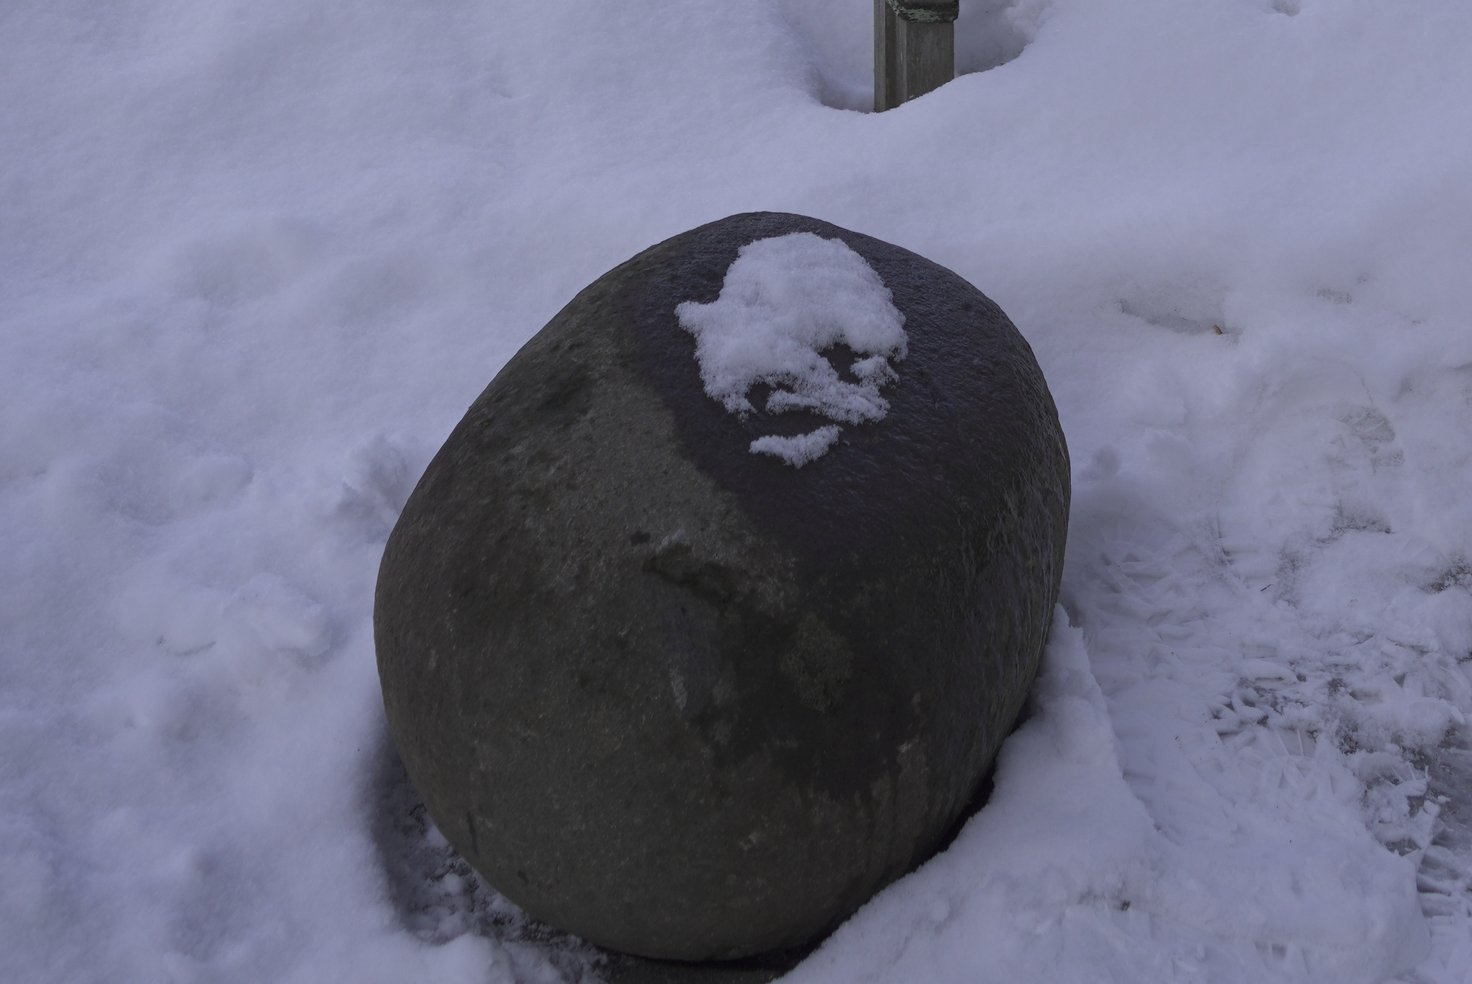
\includegraphics[width=\paperwidth]{L02/07172_about_banmochi_ishi_strength_and_grip_testing.JPG}};}
\begin{frame}
  \titlepage
\end{frame}

\part{Why Tests?}
\begin{frame}
  \partpage
\end{frame}


\begin{frame}
  \frametitle{Why Tests?}
  \begin{center}
    \Large Again: you have to move fast \& \\
    push a change to {\tt main} by end of day.\\[1em]
    Are you going break things? How do you know?\\[2em]
    \Huge \alert{State of industry: \\ run the test suite!}
  \end{center}
\end{frame}

\begin{frame}
  \frametitle{Reference}
  \begin{center}
    \Large
Kat Busch. ``A beginner's guide to automated testing.'' \\
\url{https://hackernoon.com/treat-yourself-e55a7c522f71}
  \end{center}
\end{frame}

\begin{frame}
  \frametitle{Experience report}
  \begin{center}
    
\includegraphics[width=.6\paperwidth]{L02/Dropbox_logo_2017.png} \\
  \end{center}
  \begin{changemargin}{2em}
    \large
    To pass code review: needed tests.\\[0.5em]
    ``Lo and behold, I soon needed to fix a small bug.'' \\[1em]
  \end{changemargin}

  \begin{quote}
I ran the tests. Within a few seconds, I knew that everything still worked! Not just a single code path (as in a manual test), but all code paths for which I’d written tests! It was magical. It was so much faster than my manual testing. And I knew I didn’t forget to test any edge cases, since they were all still covered in the automated tests.
\end{quote}

\end{frame}

\begin{frame}
  \frametitle{More quotes}
  \begin{changemargin}{2em}
    \Large
\begin{quote}
If your code is still in the codebase a year (or five) after you've
committed it and there are no tests for it, bugs will creep in and
nobody will notice for a long time.\\[1em]
\end{quote}

\begin{quote}
\textbf{If it matters that the code works you should write a test for it.} There is no other way you can guarantee it will work.
\end{quote}

(We'll look at other ways in this course, but tests are the state of the industry.)

  \end{changemargin}
\end{frame}

\usebackgroundtemplate{\tikz\node[opacity=0.5]{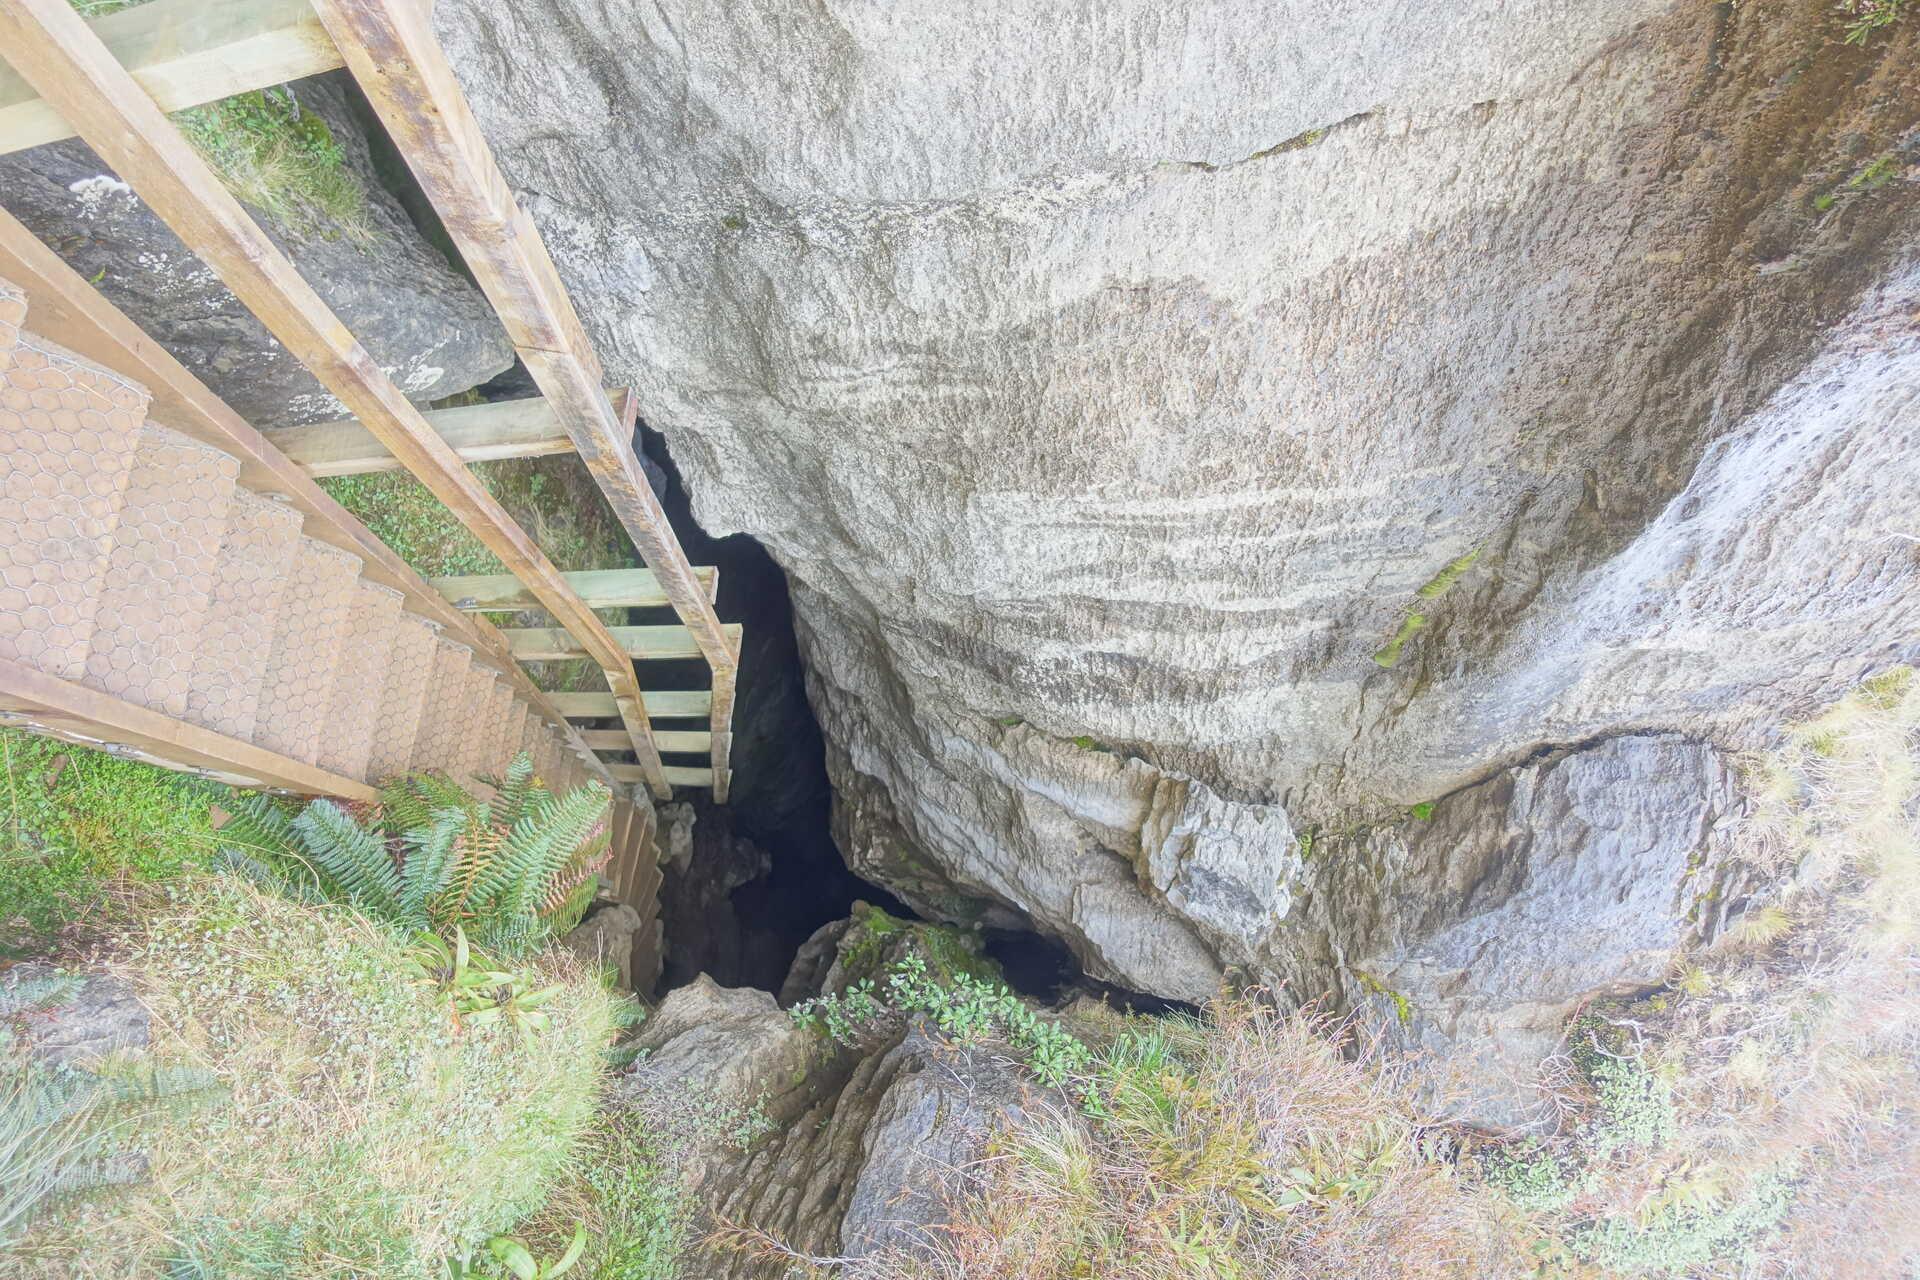
\includegraphics[width=\paperwidth]{L02/00245_into_the_cave.JPG}};}
\part{Exploratory Testing}
\begin{frame}
  \partpage
\end{frame}

\usebackgroundtemplate{\tikz\node[opacity=0.1]{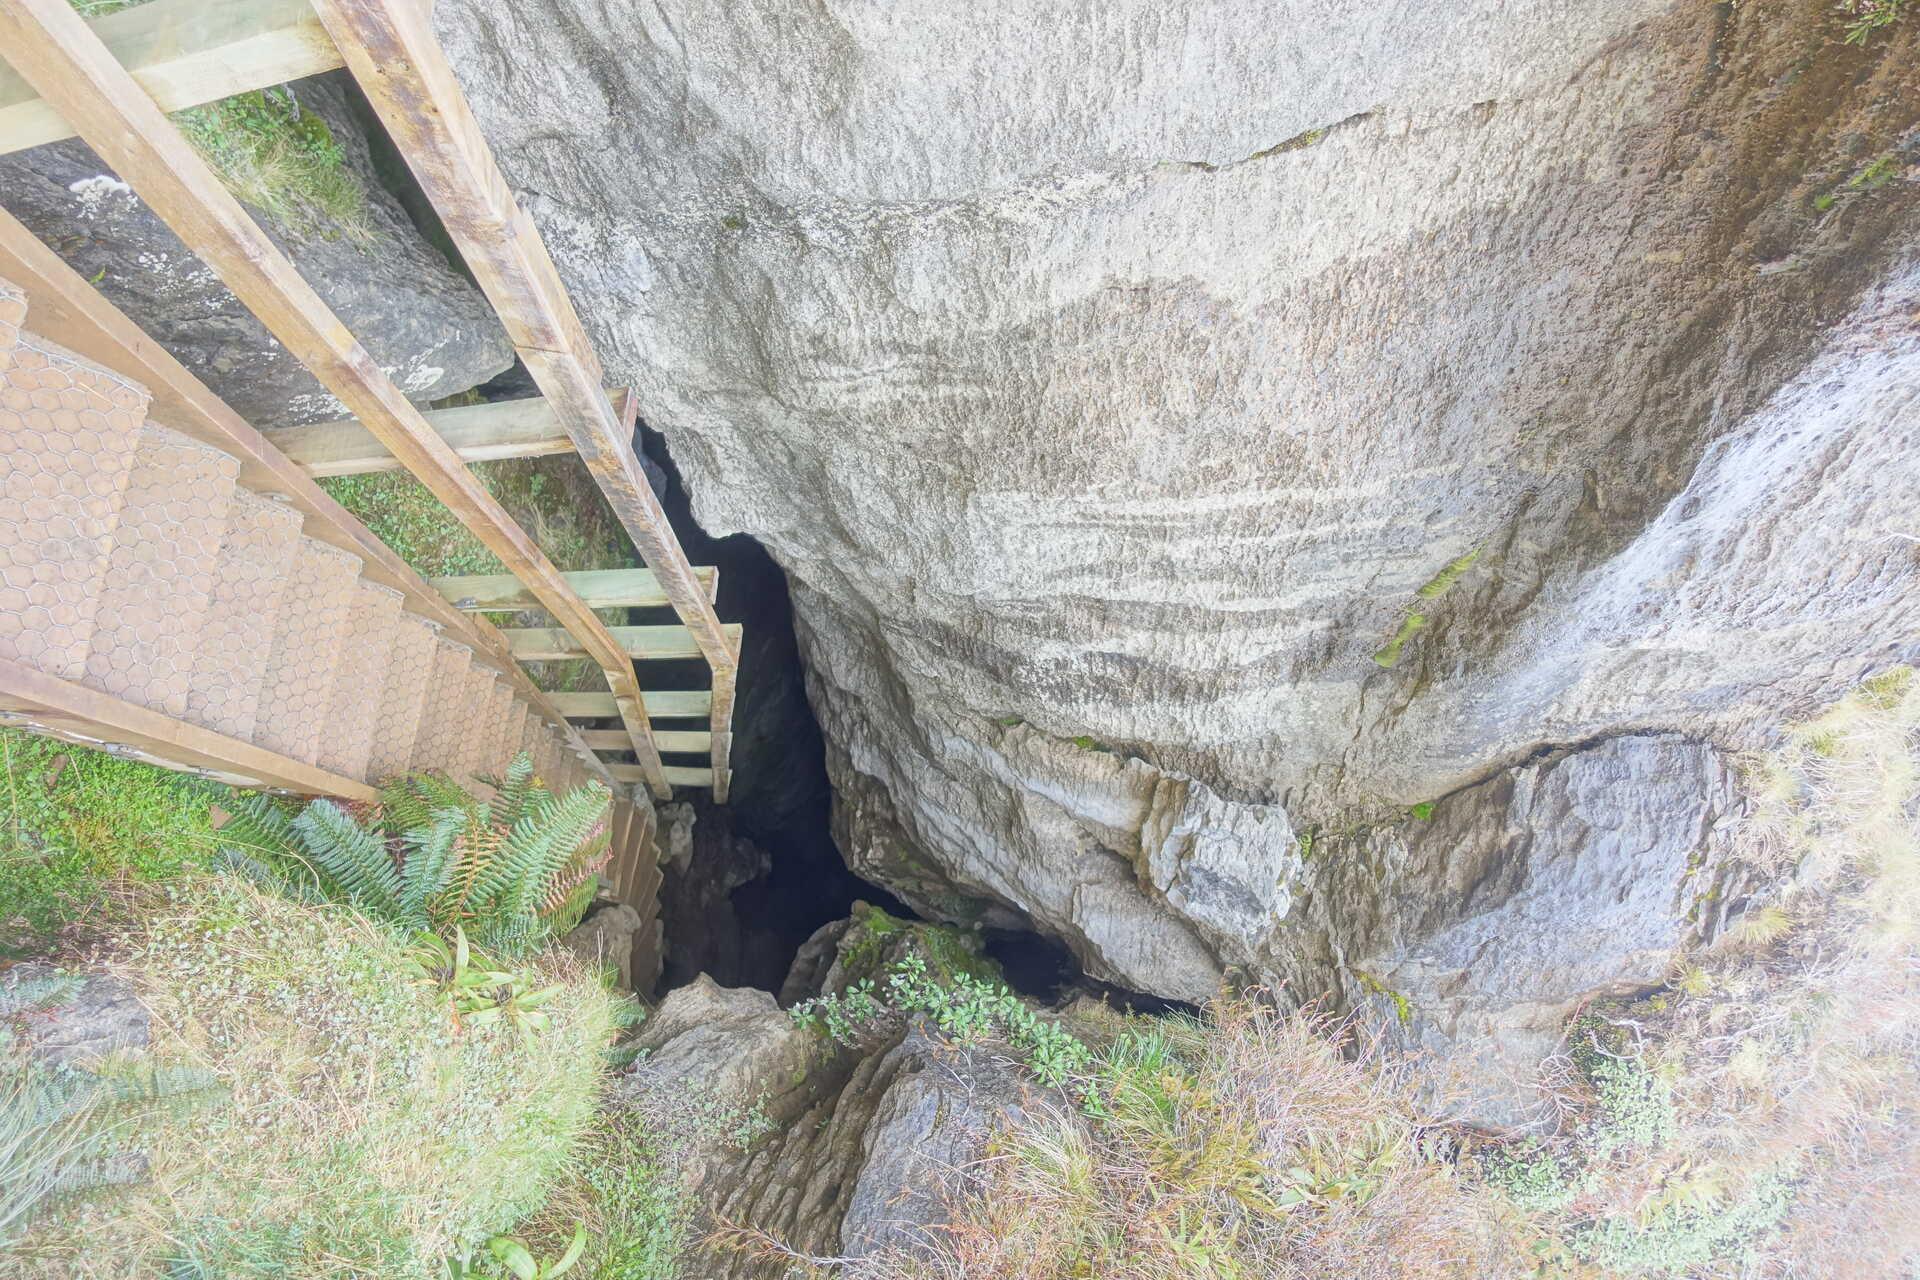
\includegraphics[width=\paperwidth]{L02/00245_into_the_cave.JPG}};}
\begin{frame}
  \frametitle{Exploratory Testing}
  \begin{changemargin}{2em}
    \Large
    Different from other testing and verification activities in this course.
    \begin{itemize}
    \item usually done by dedicated testers, not developers;
      \item but, you may do ``hallway usability testing''.
    \end{itemize}

    ~\\[0.5em]
    References in long-form notes.
  \end{changemargin}
\end{frame}

\begin{frame}
  \frametitle{Exploratory Testing Scenarios}
  \begin{changemargin}{2em}
    \begin{itemize}
      \item providing rapid feedback on new product/feature;
\item learning product quickly;
\item diversifying testing beyond scripts;
\item finding single most important bug in shortest time;
\item independent investigation of another tester's work;
\item investigating and isolating a particular defect;
\item investigate status of a particular risk to evaluate need for scripted tests.
    \end{itemize}
  \end{changemargin}
\end{frame}

\begin{frame}
  \frametitle{Exploratory Testing Process}
  \begin{changemargin}{2em}
    \begin{itemize}
    \item Start with a charter for your testing activity,\\
      \qquad ``Explore and analyze the product elements.'' \\
      \qquad These charters should be somewhat ambiguous.
\item Decide what area of the software to test.
\item Design a test (informally).
\item Execute the test; log bugs.
\item Repeat.
    \end{itemize}
  \end{changemargin}
\end{frame}

\begin{frame}
  \frametitle{Output from Exploratory Testing}
  \begin{changemargin}{2em}
    \Large
    \begin{itemize}
    \item a set of bug reports;
    \item test notes: overall impressions \& summary of test strategy / thought process;
    \item artifacts like test data / test materials (also serve as exploratory testing inputs)
    \end{itemize}
  \end{changemargin}
\end{frame}

\begin{frame}
  \frametitle{In-class exercise: Exploratory testing of WaterlooWorks [5min]}
  \begin{changemargin}{2em}
    Charter: ``Explore the overall functionality of WaterlooWorks''.
    \begin{itemize}
    \item Summarize what the purpose of WaterlooWorks is.
    \item Identify the tests that WaterlooWorks should be able to do; primary or contributing?
    \item Identify areas of potential instability.
    \item Test each function and record results (bugs).
    \end{itemize}
    PS: don't do things with actual real-world effects; \\
    normally you'd test on dev not prod.
  \end{changemargin}
\end{frame}

\part{Regression Testing}
\begin{frame}
  \partpage
\end{frame}

\begin{frame}
  \frametitle{Why Regression Tests?}
  \begin{changemargin}{2em}
    \Large
    People hate regressions. \\
    So, aim to detect regressions:
    \begin{itemize}
\item of fixed bugs;
\item in related and unrelated other features.\\[1em]
    \end{itemize}
    Usually this is integration-level testing.
  \end{changemargin}
\end{frame}

\begin{frame}
  \frametitle{Properties of Regression Tests}
  \begin{changemargin}{1em}
    \Large
    \begin{itemize}
    \item automated! \\ \qquad (usually low-yield)
    \item appropriately sized\\ \qquad (should be part of continuous integration)
    \item up-to-date
    \end{itemize}
  \end{changemargin}
\end{frame}

\begin{frame}
  \frametitle{Automating Regression Tests}
  \begin{changemargin}{1em}
    \Large
    Pretty easy when it's e.g. a compiler. \\
    Otherwise, not so easy.\\[1em]
    Input:
    \begin{itemize}
    \item from a file?
    \item webform submissions?
    \item interacting with a webpage?\\[.5em]
    \end{itemize}
    Approaches for non-file inputs:
    \begin{itemize}
      \item special mocks to take file-based inputs;
      \item capture and replay events (e.g. Selenium).
    \end{itemize}
  \end{changemargin}
\end{frame}

\begin{frame}
  \frametitle{Automating Regression Tests: Output}
  \begin{changemargin}{1em}
    \Large
    How to verify output? Can be hard!\\
    resolution, whitespace, window placement\ldots\\[1em]

    Case study: Gecko (used in Firefox, Thunderbird).
    \begin{enumerate}
    \item manual testers
    \item capture screenshots, compare (often failed)
    \item enable logging, compare logs.
    \end{enumerate}
  \end{changemargin}
\end{frame}

\begin{frame}
  \frametitle{Some Industrial Best Practices}
  \begin{changemargin}{2em}
    \Large
    What have you seen?
  \end{changemargin}
\end{frame}

\begin{frame}
  \frametitle{Some Industrial Best Practices}
  \begin{changemargin}{1em}
    \Large
    \begin{itemize}
    \item unit tests
    \item code reviews
    \item continuous builds
    \item one-button deploy
    \item undo/back button
    \end{itemize}
  \end{changemargin}
\end{frame}

\usebackgroundtemplate{\tikz\node[opacity=0.5]{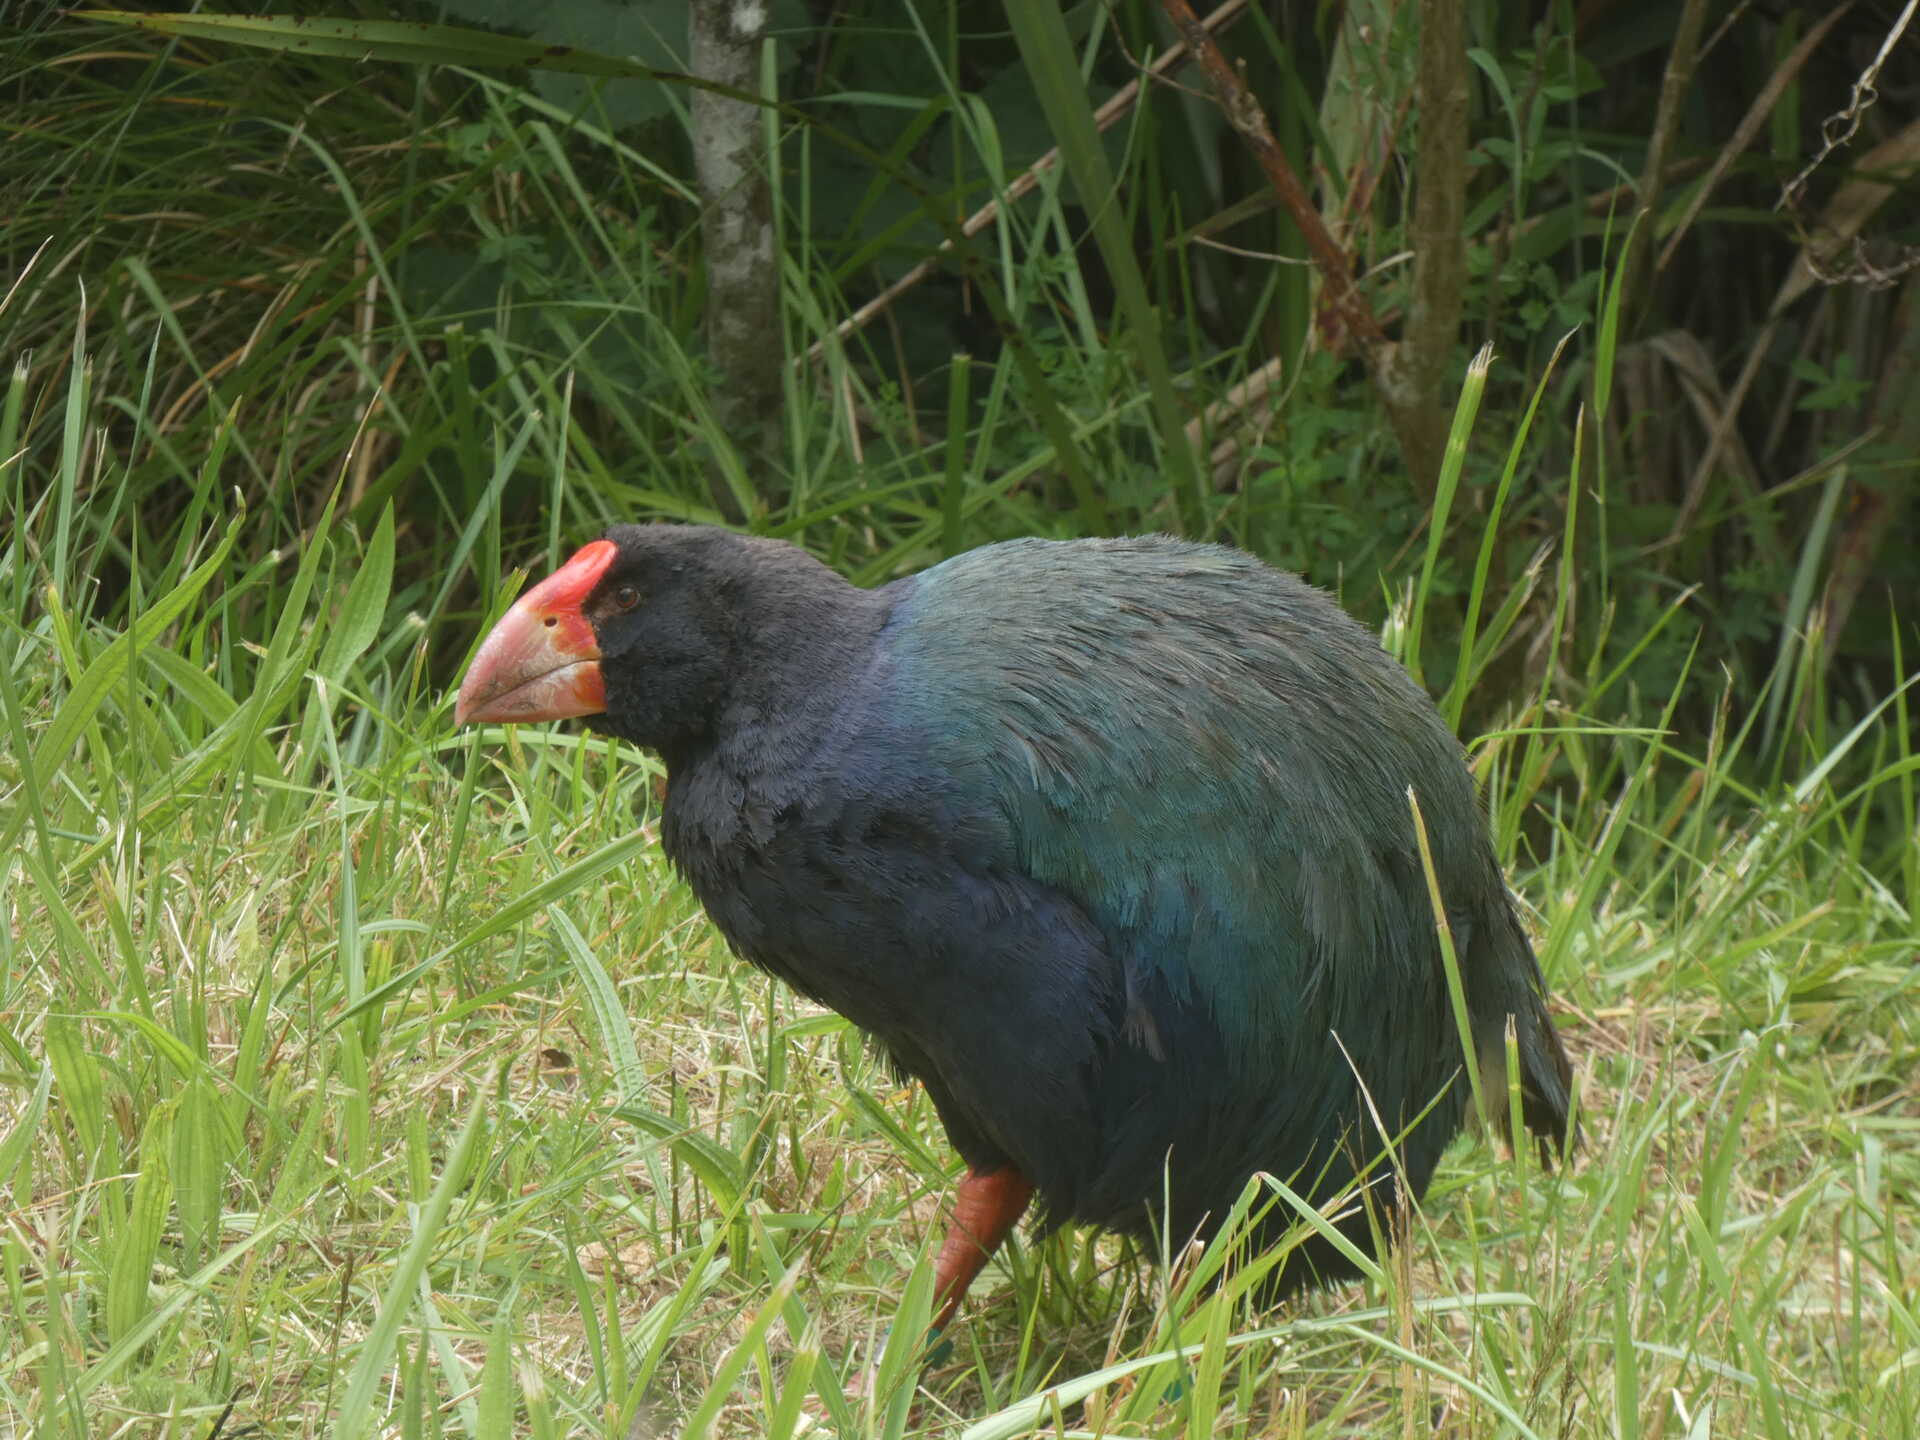
\includegraphics[width=\paperwidth]{L02/90360_takahe.JPG}};}
\part{Unit Tests}
\begin{frame}
  \partpage
\end{frame}

\usebackgroundtemplate{\tikz\node[opacity=0.1]{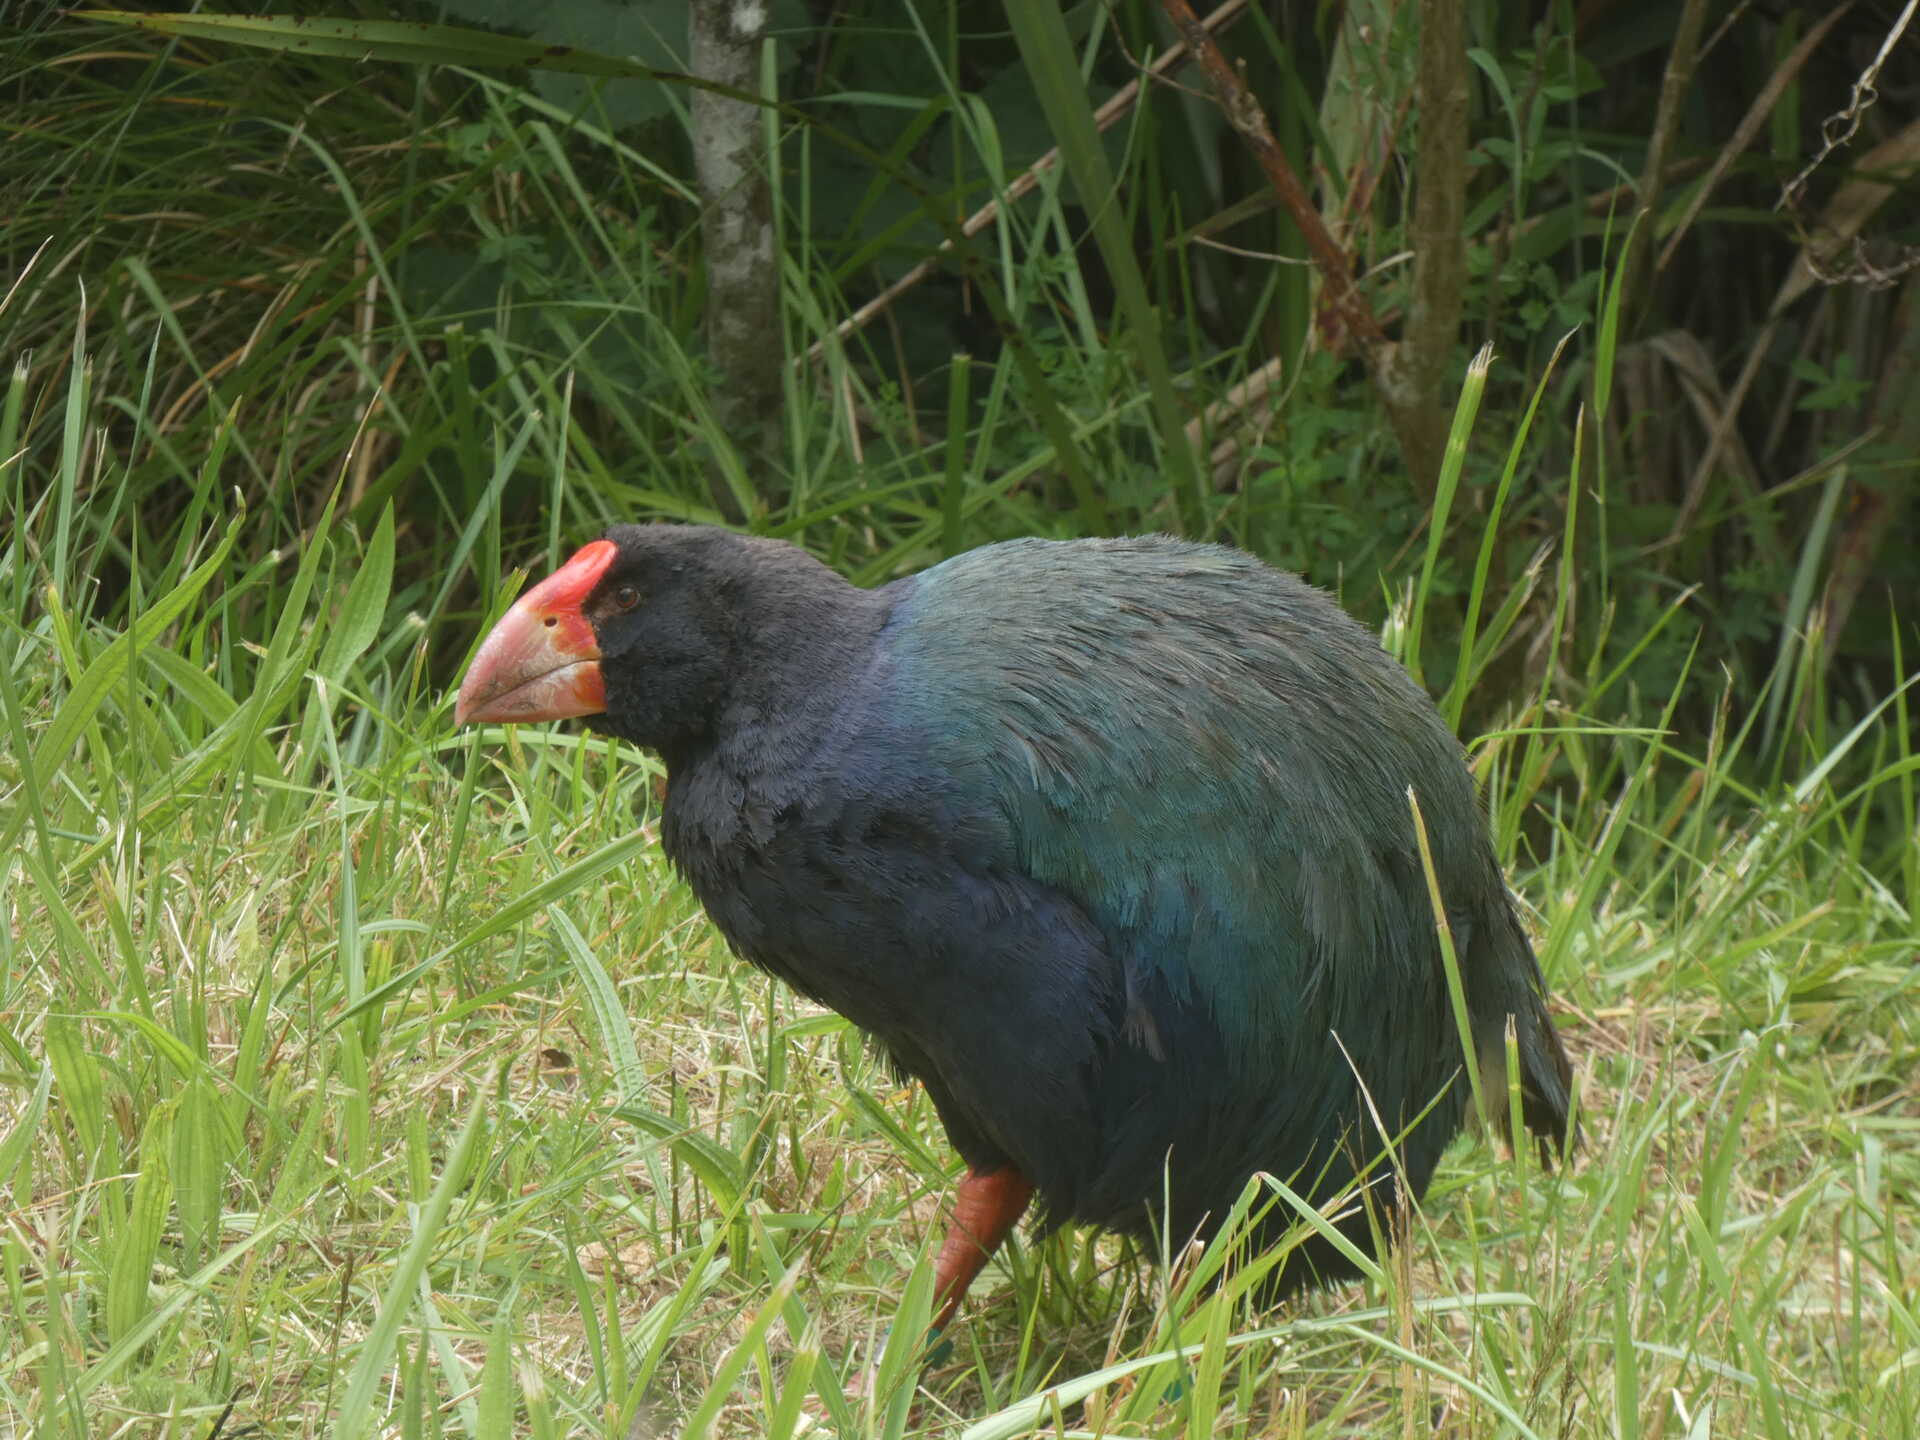
\includegraphics[width=\paperwidth]{L02/90360_takahe.JPG}};}

\begin{frame}
  \frametitle{About Unit Tests}
  \begin{changemargin}{2em}
    \Large
    \begin{itemize}
    \item focus on one particular class, module or function;
    \item should execute quickly;
    \item may need fake inputs or mocks;
    \item should generally not use an entire real input for a unit test.
    \end{itemize}
  \end{changemargin}
\end{frame}

\begin{frame}[fragile]
  \frametitle{An Example Unit Test}
  \begin{changemargin}{1em}

    {\Large
      This example is JUnit; many other frameworks exist.\\[1em]
      }
    
    \begin{lstlisting}[]
    @Test
    public void testFindLast() {
        int[] x = new int[] {2, 3, 5}; // arrange
        int last = FindLast.findLast(x, 2); // act
        assertEquals(0, last); // assert
    }
\end{lstlisting}

  \end{changemargin}
\end{frame}

\begin{frame}[fragile]
  \frametitle{More Pro-Test Propaganda}
  \begin{changemargin}{1em}

    {\Large
\begin{quote}
You'll find that writing tests as you go makes your interfaces better and makes your code more testable. If you find yourself writing something hard to test, you'll notice it early on when there's still time to improve the design.
\end{quote}
}
  \end{changemargin}
\end{frame}
\begin{frame}
  \frametitle{Goal}

  \Large
  \begin{changemargin}{2cm}
    Good tests are \emph{self-checking}:\\[1em]
    no errors, no failures = successful test.
  \end{changemargin}

  \begin{center}
    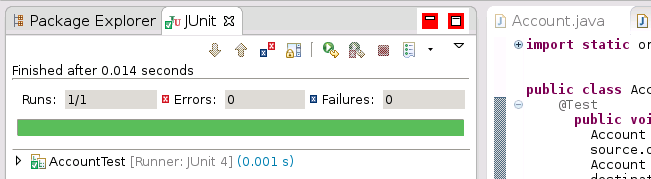
\includegraphics[width=.6\textwidth]{L02/pass}
  \end{center}
  
\end{frame}

\begin{frame}
  \frametitle{Why Self-Checking Tests?}

  \Large
  \begin{changemargin}{2cm}
    Tests automatically report status.\\[1em]
    Enables ``keep the bar green''\\
    coding style.\\[1em]
    Worry less about introducing bugs.\\[1em]
    Plus: Tests help document system specs.
  \end{changemargin}
\end{frame}

\begin{frame}
  \frametitle{Plan}

  \Large
  \begin{changemargin}{1cm}
    HOWTO make your tests self-checking.
  \end{changemargin}
\end{frame}

\begin{frame}
  \Large
  \begin{changemargin}{2cm}
    ``Isn't it just calling asserts?''\\[1em]
\only<2>{    \hspace*{4cm} [sadly, no.]}
  \end{changemargin}
\end{frame}

\begin{frame}
  \Large
  \begin{changemargin}{2cm}
    Two questions about asserts:
    \begin{enumerate}
    \item Q: what for?\\
      A: check method call results\\[1em]
    \item Q: where?\\
      A: usually after calling SUT \\ ~~~~(System Under Test)
    \end{enumerate}
  \end{changemargin}
\end{frame}

\begin{frame}
  \frametitle{Counter Example}

  \begin{changemargin}{0.5cm}
    \lstinputlisting{L02/Counter.java}
  \end{changemargin}
\end{frame}

\begin{frame}
  \frametitle{Counter Test}

  \begin{changemargin}{0.5cm}
    \lstinputlisting{L02/CounterTest.java}
  \end{changemargin}
\end{frame}

\begin{frame}
  \frametitle{State or Behaviour?}

  \begin{changemargin}{2cm}
    Was Counter Test verifying state or behaviour?
  \end{changemargin}
\end{frame}

\begin{frame}
  \frametitle{State vs Behaviour}

  \large
  \begin{changemargin}{2cm}
    {\bf State:} e.g. object field values.\\
    \hspace*{1.5cm}
    Call accessor methods to verify.\\[1em]
    {\bf Behaviour:} which calls SUT makes.\\
    \hspace*{1.5cm} Insert observation points, \\ \hspace*{1.5cm} monitor interactions.
  \end{changemargin}
\end{frame}

\begin{frame}
  \frametitle{Flight example}

  \small
    \lstinputlisting{L02/flight.java}
\end{frame}

\begin{frame}
  \frametitle{Flight example: state verification}

  \small
    \lstinputlisting{L02/flight_extended_state_spec.java}
\end{frame}

\begin{frame}
  \frametitle{What Is State Verification?}

  \Large
  \begin{changemargin}{2cm}
    \begin{enumerate}
    \item Exercise SUT.
    \item Verify state \& check return values.
    \end{enumerate}

    ~\\[1em]
    Inspect only outputs; \\ \hspace*{1cm} only call methods from SUT.\\[1em]
    Do not instrument SUT.\\[1em]
    Do not check interactions.
  \end{changemargin}
\end{frame}

\begin{frame}
  \frametitle{Implementing State Verification}

  \Large
  \begin{changemargin}{2cm}
    Two options:
    \begin{enumerate}
    \item procedural (bunch of asserts); or,
    \item via expected objects (won't talk about them this year).
    \end{enumerate}
  \end{changemargin}
\end{frame}

\begin{frame}
  \frametitle{Flight Example: discussing state verification}

  \large
  \begin{changemargin}{2cm}
    We do check that the flight got removed.\\
    We don't check that the removal got logged.\\[1em]
    Hard to check state and observe logging.\\[1em]
    Solution: Spy on SUT behaviour.
  \end{changemargin}
\end{frame}


\begin{frame}
  \frametitle{Flight example: procedural behaviour verification}

  \small
    \lstinputlisting{L02/flight_pbv.java}
\end{frame}

\begin{frame}
  \frametitle{Alternative: Expected Behaviour Specification}
  \Large
  \begin{changemargin}{2cm}
    Use a mock object framework (e.g. JMock)\\
    to define expected behaviour.\\[1em]

    Observe calls to the logger, \\
    make sure right calls happen.
  \end{changemargin}
\end{frame}

\begin{frame}
  \frametitle{Kinds of Assertions}
  \large
  \begin{changemargin}{2cm}
    Three built-in choices:
    \begin{enumerate}
    \item assertTrue(aBooleanExpression)
    \item assertEquals(expected, actual)
    \item assertEquals(expected, actual, tolerance)
    \end{enumerate}
    ~\\[1em]
    note: {\tt assertTrue} can give \\
    hard-to-diagnose error messages \\
    (must try harder when using).
  \end{changemargin}
\end{frame}

\begin{frame}
  \frametitle{Using Assertions}
  \large
  \begin{changemargin}{2cm}
    Assertions are good:
    \begin{itemize}
    \item to check all things that should be true\\
      \begin{changemargin}{1cm}
        (more = better)
      \end{changemargin}
    \item to serve as documentation:
      \begin{changemargin}{1cm}
        when system in state $S_1$,\\
        and I do $X$,\\
        assert that the result should be $R$, and\\
        that system should be in $S_2$.
      \end{changemargin}
    \item to allow failure diagnosis\\
            \begin{changemargin}{1cm}
              (include assertion messages!)
            \end{changemargin}
    \end{itemize}
  \end{changemargin}
\end{frame}

\begin{frame}
  \frametitle{Not Using Assertions}
  \Large
  \begin{changemargin}{2cm}
    Can also do external result verification:\\[1em]
    Write output to files, diff (or custom diff)
    expected and actual output.\\[1em]
    Twist: expected result then not visible when looking at test.\\[1em]
    (What's a good workaround?)
  \end{changemargin}
\end{frame}

\begin{frame}
  \frametitle{Verifying Behaviour}
  \Large
  \begin{changemargin}{2cm}
    Observe actions (calls) of the SUT.
    \begin{itemize}
    \item procedural behaviour verification; or,\\
      (challenge: recording \& verifying behaviour)\\[.5em]
    \item via expected behaviour specification.\\
      (also captures outbound calls of SUT)
    \end{itemize}
  \end{changemargin}
\end{frame}

\usebackgroundtemplate{\tikz\node[opacity=0.2]{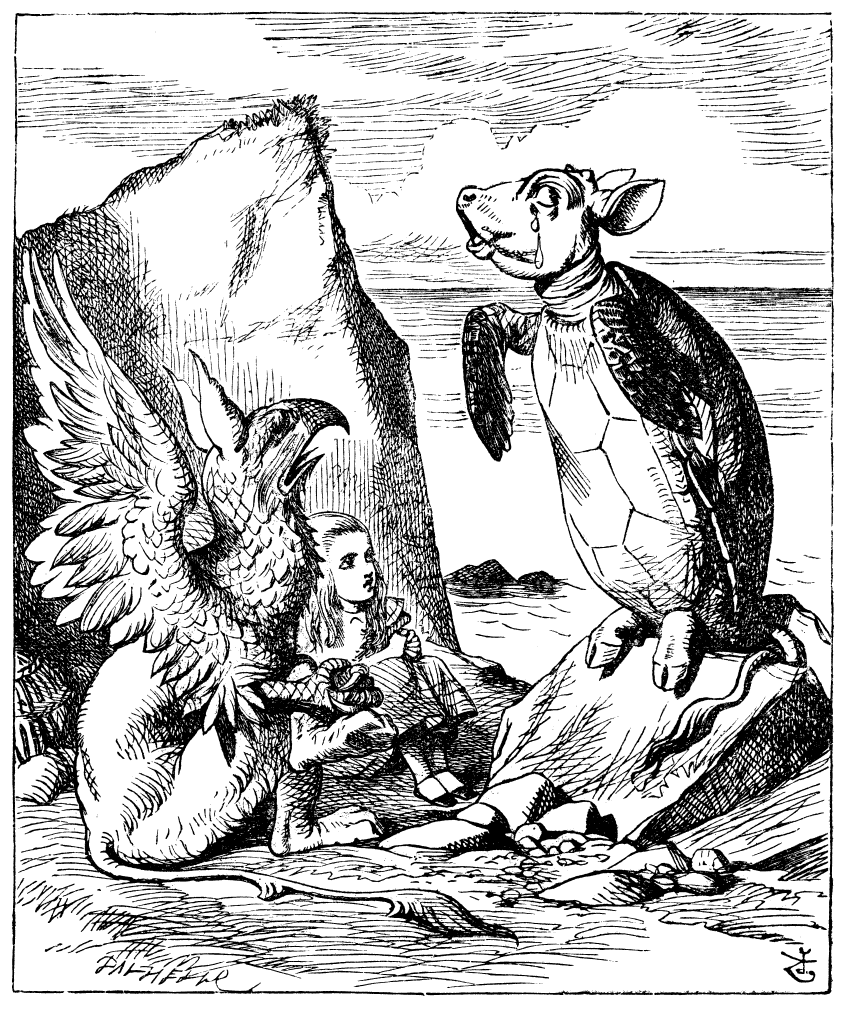
\includegraphics[width=\paperwidth]{L02/Alice_par_John_Tenniel_34.png}};}
\part{Mock Objects}
\begin{frame}
  \partpage
  \vspace*{.45\textheight}
  \begin{center}
    John Tenniel's original (1865) illustration for Lewis Carroll's ``Alice in Wonderland''. Alice sitting between Gryphon and Mock turtle.
  \end{center}
\end{frame}


\usebackgroundtemplate{\tikz\node[opacity=0.03]{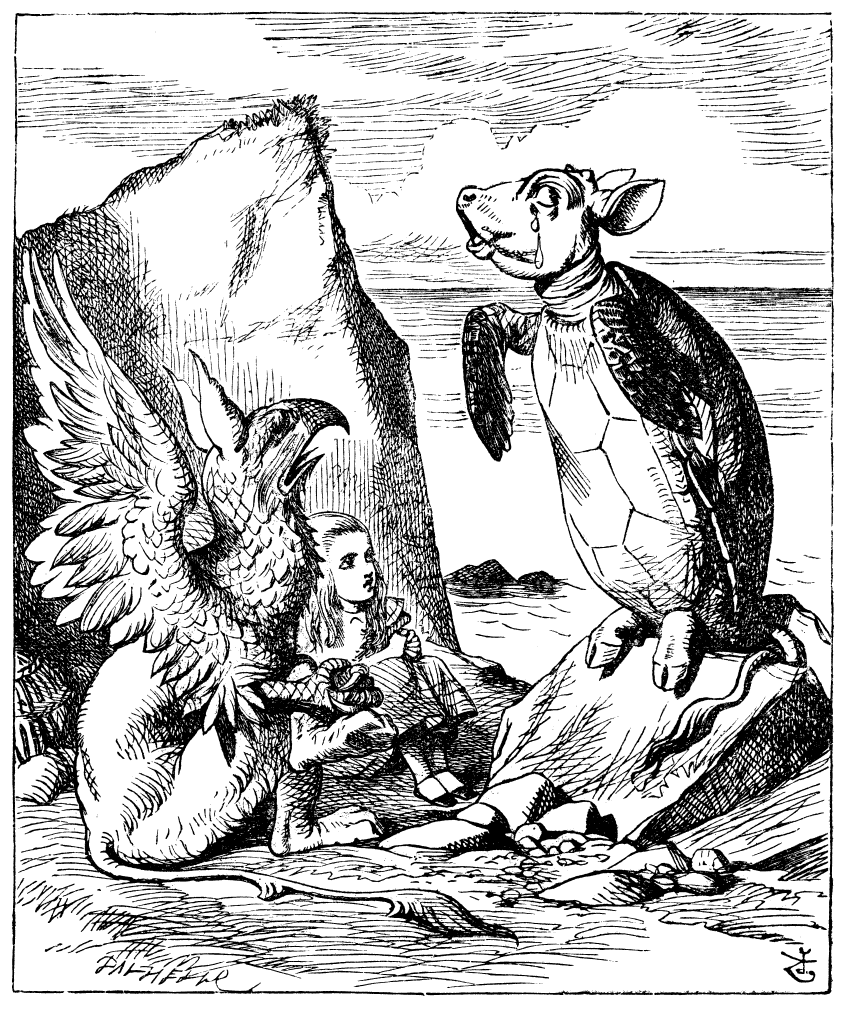
\includegraphics[width=\paperwidth]{L02/Alice_par_John_Tenniel_34.png}};}
\begin{frame}[fragile]
  \frametitle{Mock Objects: Email Sender}
  \begin{changemargin}{1cm}
{\small
  \begin{lstlisting}
  // state or behaviour verification?
  public class MailServiceStub
                 implements MailService {
    private List<Message> messages =
        new ArrayList<Message>();
    
    public void send (Message msg) {
      messages.add(msg);
    }
    public int numberSent() {
      return messages.size();
    }
  }     
\end{lstlisting}
}
  \end{changemargin}
\end{frame}

\begin{frame}[fragile]
  \frametitle{Mock Objects: Behaviour Verification}
  \begin{changemargin}{1cm}
{\small
  \begin{lstlisting}
// jMock syntax
class OrderInteractionTester... {
  public void testOrderSendsMailIfUnfilled() {
    Order order = new Order(TALISKER, 51);
    Mock warehouse = mock(Warehouse.class); // (1)
    Mock mailer = mock(MailService.class);
    order.setMailer((MailService) mailer.proxy());

    mailer.expects(once()).method("send"); // (2)
    warehouse.expects(once()).method("hasInventory")
      .withAnyArguments()
      .will(returnValue(false));

    order.fill((Warehouse) warehouse.proxy());
  }
}    
\end{lstlisting}
}
  \end{changemargin}
\end{frame}

\begin{frame}[fragile]
  \frametitle{Mock Objects: Document Management}
  \begin{changemargin}{1cm}
{\small
  \begin{lstlisting}
// EasyMock syntax
@RunWith(EasyMockRunner.class)
public class ExampleTest {
  @TestSubject
  private ClassUnderTest classUnderTest =
      new ClassUnderTest();

  @Mock // creates a mock object
  private Collaborator mock;

  @Test
  public void testRemoveNonExistingDocument() {
    replay(mock);
    classUnderTest.removeDocument
        ("Does not exist");
  }
} 
\end{lstlisting}
}
  \end{changemargin}
\end{frame}

\begin{frame}[fragile]
  \frametitle{Mock Objects: Using a Mock}
  \begin{changemargin}{1cm}
{\small
  \begin{lstlisting}
@Test
public void testAddDocument() {
  // ** recording phase **
  // expect document addition
  mock.documentAdded("Document");
  // expect to be asked to vote for document removal, and vote for it
  expect(mock.voteForRemoval("Document"))
             .andReturn((byte) 42);
  // expect document removal
  mock.documentRemoved("Document");
  replay(mock);
  // ** replaying phase **
  // we expect the recorded actions to happen
  classUnderTest.addDocument("New Document",
      new byte[0]);
  // check that the behaviour actually happened:
  verify(mock);
  \end{lstlisting}
}
  \end{changemargin}
\end{frame}

\usebackgroundtemplate{\tikz\node[opacity=0.4]{
\includegraphics[width=\paperwidth]{L02/croissant-410322_1920.jpg}};}
\part{Flakiness: Good for croissants, bad for tests}
\begin{frame}
  \partpage
  \begin{center}
    (thanks Pixabay for the picture)
  \end{center}
\end{frame}

\usebackgroundtemplate{\tikz\node[opacity=0.1]{
\includegraphics[width=\paperwidth]{L02/croissant-410322_1920.jpg}};}
\begin{frame}[fragile]
  \frametitle{Dealing with Flakiness}
  \Large
  \begin{changemargin}{1cm}
    There are mitigations:
    \begin{itemize}
    \item label known-flaky tests and rerun them
    \item ignore or remove flaky tests
    \end{itemize}
    They're not great. \\
    Takes a long time to re-run tests.
  \end{changemargin}
\end{frame}

\begin{frame}[fragile]
  \frametitle{Causes of Flakiness}
  \Large
  \begin{changemargin}{1cm}
    Luo et al studied 201 fixes to flaky tests in open-source projects. Fixable causes:
    \begin{itemize}
    \item improper waits for asynchronous responses;
    \item concurrency; and
    \item test order dependency.
    \end{itemize}
  \end{changemargin}
\end{frame}

\begin{frame}[fragile]
  \frametitle{Asynchronous waits}
  \Large
  \begin{changemargin}{1cm}
    Typically: a \texttt{sleep()} call which didn't wait long enough.\\[1em]
    Best practice:
    \begin{itemize}
      \item use some sort of \texttt{wait()} call to wait for the result,
        instead of hardcoding a sleep time.
    \end{itemize}
  \end{changemargin}
\end{frame}

\begin{frame}[fragile]
  \frametitle{Concurrency}
  \Large
  \begin{changemargin}{1cm}
    The usual (see CS343 for more):
    \begin{itemize}
    \item data races;
    \item atomicity violations;
    \item deadlocks.
    \end{itemize}
  \end{changemargin}
\end{frame}

\begin{frame}[fragile]
  \frametitle{Test order dependency}
  \Large
  \begin{changemargin}{1cm}
    \begin{itemize}
    \item Test A expects test B to have already executed \\
      (and to have left a side effect, e.g. a file).\\[1em]
    \end{itemize}
    Especially common in the transition from Java 6 to Java 7,
    because the test execution order changed.\\[1em]
    Solution: remove the dependency.
  \end{changemargin}
\end{frame}

  \end{document}
